\documentclass[11pt]{article}

\usepackage[margin=1in]{geometry}
\usepackage[T1]{fontenc}
\usepackage{graphicx}
\usepackage{longtable}
\usepackage{booktabs}
\usepackage{array}
\usepackage{enumitem}
\usepackage{xcolor}
\usepackage{hyperref}
\usepackage{tikz}
\usepackage{float}
\usepackage{fancyhdr}
\usepackage{titlesec}
\usepackage{tcolorbox}
\usepackage{tabularx}
\usepackage{multirow}
\usepackage{caption}
\usepackage{makecell}
\usepackage{amssymb}
\usepackage{pifont}

\usetikzlibrary{shapes.geometric, arrows.meta, positioning, fit, backgrounds, calc, decorations.pathreplacing, shapes.multipart, matrix, shadows}

% ---------------------------------------------------------------------------
% Color Definitions
% ---------------------------------------------------------------------------
\definecolor{sectionblue}{RGB}{31,78,121}
\definecolor{rwcolor}{RGB}{153,50,204}
\definecolor{vbcolor}{RGB}{60,179,113}
\definecolor{funccolor}{RGB}{70,130,180}
\definecolor{infocolor}{RGB}{255,165,0}
\definecolor{conccolor}{RGB}{220,53,69}
\definecolor{devcolor}{RGB}{60,179,113}
\definecolor{deploycolor}{RGB}{255,127,80}
\definecolor{opscolor}{RGB}{128,128,128}
\definecolor{flowcolor}{RGB}{100,100,100}
\definecolor{lightgray}{RGB}{245,245,245}
\definecolor{warningred}{RGB}{220,53,69}
\definecolor{successgreen}{RGB}{40,167,69}
\definecolor{infoblue}{RGB}{23,162,184}
\definecolor{perspcolor}{RGB}{186,85,211}
\definecolor{modulecolor}{RGB}{144,238,144}
\definecolor{cnccolor}{RGB}{255,182,193}
\definecolor{alloccolor}{RGB}{173,216,230}

\hypersetup{
  colorlinks=true,
  linkcolor=sectionblue,
  urlcolor=sectionblue,
  citecolor=sectionblue
}

% ---------------------------------------------------------------------------
% Header and Footer
% ---------------------------------------------------------------------------
\pagestyle{fancy}
\fancyhf{}
\fancyhead[L]{\leftmark}
\fancyhead[R]{Rozanski \& Woods / Views \& Beyond Integration}
\fancyfoot[C]{\thepage}
\renewcommand{\headrulewidth}{0.4pt}
\renewcommand{\footrulewidth}{0.4pt}

% ---------------------------------------------------------------------------
% Section Formatting
% ---------------------------------------------------------------------------
\titleformat{\section}
  {\normalfont\Large\bfseries\color{sectionblue}}{\thesection}{1em}{}
\titleformat{\subsection}
  {\normalfont\large\bfseries\color{sectionblue!80}}{\thesubsection}{1em}{}
\titleformat{\subsubsection}
  {\normalfont\normalsize\bfseries\color{sectionblue!60}}{\thesubsubsection}{1em}{}

% ---------------------------------------------------------------------------
% Custom Box Environments
% ---------------------------------------------------------------------------
\newtcolorbox{keypoint}{
    colback=blue!5,
    colframe=sectionblue,
    title=Key Point,
    fonttitle=\bfseries
}

\newtcolorbox{warning}{
    colback=red!5,
    colframe=warningred,
    title=Warning,
    fonttitle=\bfseries
}

\newtcolorbox{bestpractice}{
    colback=green!5,
    colframe=successgreen,
    title=Best Practice,
    fonttitle=\bfseries
}

\newtcolorbox{example}{
    colback=lightgray,
    colframe=flowcolor,
    title=Example,
    fonttitle=\bfseries
}

\newtcolorbox{definition}{
    colback=infoblue!10,
    colframe=infoblue,
    title=Definition,
    fonttitle=\bfseries
}

\newtcolorbox{rwbox}[1][]{
    colback=rwcolor!8,
    colframe=rwcolor,
    title=#1,
    fonttitle=\bfseries,
    breakable
}

\newtcolorbox{vbbox}[1][]{
    colback=vbcolor!10,
    colframe=vbcolor,
    title=#1,
    fonttitle=\bfseries,
    breakable
}

\newtcolorbox{mappingbox}[1][]{
    colback=infocolor!10,
    colframe=infocolor,
    title=#1,
    fonttitle=\bfseries
}

\newtcolorbox{perspbox}[1][]{
    colback=perspcolor!10,
    colframe=perspcolor,
    title=#1,
    fonttitle=\bfseries
}

\newtcolorbox{checklistbox}[1][]{
    colback=white,
    colframe=flowcolor,
    title=#1,
    fonttitle=\bfseries
}

\tcbuselibrary{listings,breakable}

% ---------------------------------------------------------------------------
% List Settings
% ---------------------------------------------------------------------------
\setlist[itemize]{leftmargin=*,topsep=3pt,itemsep=2pt,parsep=0pt}
\setlist[enumerate]{leftmargin=*,topsep=3pt,itemsep=2pt,parsep=0pt}

% ---------------------------------------------------------------------------
% Custom Column Types
% ---------------------------------------------------------------------------
\newcolumntype{L}[1]{>{\raggedright\arraybackslash}p{#1}}
\newcolumntype{C}[1]{>{\centering\arraybackslash}p{#1}}
\newcolumntype{R}[1]{>{\raggedleft\arraybackslash}p{#1}}

% ---------------------------------------------------------------------------
% Custom Commands
% ---------------------------------------------------------------------------
\newcommand{\rw}{Rozanski \& Woods}
\newcommand{\vb}{Views \& Beyond}
\newcommand{\funcview}{\textcolor{funccolor}{\textbf{Functional}}}
\newcommand{\infoview}{\textcolor{infocolor}{\textbf{Information}}}
\newcommand{\concview}{\textcolor{conccolor}{\textbf{Concurrency}}}
\newcommand{\devview}{\textcolor{devcolor}{\textbf{Development}}}
\newcommand{\deployview}{\textcolor{deploycolor}{\textbf{Deployment}}}
\newcommand{\opsview}{\textcolor{opscolor}{\textbf{Operational}}}

% ---------------------------------------------------------------------------
% Title
% ---------------------------------------------------------------------------
\title{%
    \vspace{-1cm}
    \textbf{\Huge Software Architecture Documentation}\\[12pt]
    \Large Integrating Rozanski \& Woods with Views and Beyond\\[8pt]
    \large A Comprehensive Guide to Mapping Viewpoints,\\
    Perspectives, and Documentation Practices
}
\author{%
    \textit{Architecture Documentation Series}\\[4pt]
    \small Based on Software Systems Architecture (R\&W) and SEI Views and Beyond
}
\date{\today}

\begin{document}
\maketitle
\thispagestyle{empty}

\vspace{0.5cm}

\begin{abstract}
\noindent
Rozanski and Woods' ``Software Systems Architecture'' and the SEI's ``Views and Beyond'' represent two of the most influential approaches to software architecture documentation. While both frameworks share common foundations in IEEE 1471/ISO 42010, they offer distinct perspectives and terminology. This comprehensive guide provides detailed mappings between the six Rozanski \& Woods viewpoints and Views and Beyond view types, addresses the R\&W perspectives and their V\&B equivalents, and offers practical guidance for creating documentation that leverages the strengths of both approaches. Whether you are familiar with one framework and need to work with the other, or seeking to create documentation that satisfies multiple stakeholder communities, this guide provides the integration knowledge you need.
\end{abstract}

\vfill

\begin{center}
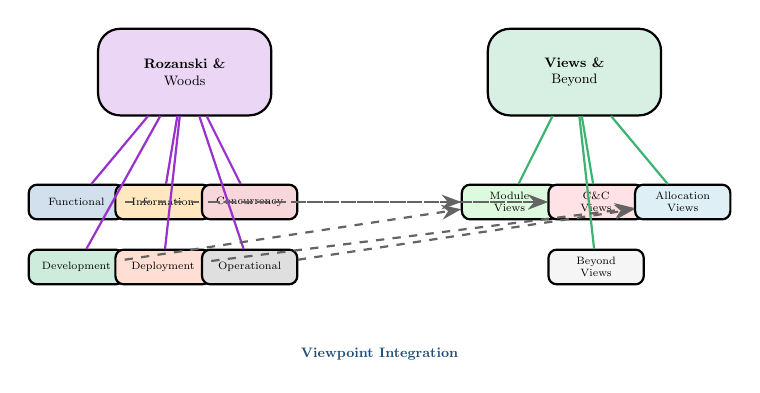
\begin{tikzpicture}[
    scale=0.55,
    transform shape,
    framework/.style={draw, thick, rounded corners=8pt, minimum width=4cm, minimum height=2cm, font=\small, align=center},
    viewpoint/.style={draw, thick, rounded corners=3pt, minimum width=2.2cm, minimum height=0.8cm, font=\scriptsize, align=center},
    arrow/.style={-{Stealth[length=2.5mm]}, thick, dashed}
]
    % R&W side
    \node[framework, fill=rwcolor!20] (rw) at (-4.5,3) {\textbf{Rozanski \&}\\Woods};
    \node[viewpoint, fill=funccolor!25] (func) at (-7,0) {Functional};
    \node[viewpoint, fill=infocolor!25] (info) at (-5,0) {Information};
    \node[viewpoint, fill=conccolor!20] (conc) at (-3,0) {Concurrency};
    \node[viewpoint, fill=devcolor!25] (dev) at (-7,-1.5) {Development};
    \node[viewpoint, fill=deploycolor!25] (deploy) at (-5,-1.5) {Deployment};
    \node[viewpoint, fill=opscolor!25] (ops) at (-3,-1.5) {Operational};
    
    % V&B side
    \node[framework, fill=vbcolor!20] (vb) at (4.5,3) {\textbf{Views \&}\\Beyond};
    \node[viewpoint, fill=modulecolor!30] (mod) at (3,0) {Module\\Views};
    \node[viewpoint, fill=cnccolor!40] (cnc) at (5,0) {C\&C\\Views};
    \node[viewpoint, fill=alloccolor!40] (alloc) at (7,0) {Allocation\\Views};
    \node[viewpoint, fill=lightgray] (beyond) at (5,-1.5) {Beyond\\Views};
    
    % Connections from frameworks
    \draw[thick, rwcolor] (rw) -- (func);
    \draw[thick, rwcolor] (rw) -- (info);
    \draw[thick, rwcolor] (rw) -- (conc);
    \draw[thick, rwcolor] (rw) -- (dev);
    \draw[thick, rwcolor] (rw) -- (deploy);
    \draw[thick, rwcolor] (rw) -- (ops);
    
    \draw[thick, vbcolor] (vb) -- (mod);
    \draw[thick, vbcolor] (vb) -- (cnc);
    \draw[thick, vbcolor] (vb) -- (alloc);
    \draw[thick, vbcolor] (vb) -- (beyond);
    
    % Mapping arrows
    \draw[arrow, flowcolor] (func) -- (cnc);
    \draw[arrow, flowcolor] (info) -- (mod);
    \draw[arrow, flowcolor] (conc) -- (cnc);
    \draw[arrow, flowcolor] (dev) -- (mod);
    \draw[arrow, flowcolor] (deploy) -- (alloc);
    \draw[arrow, flowcolor] (ops) -- (alloc);
    
    % Label
    \node[font=\bfseries\small, text=sectionblue] at (0,-3.5) {Viewpoint Integration};
\end{tikzpicture}
\end{center}

\newpage
\tableofcontents
\newpage

%==============================================================================
\section{Introduction}
%==============================================================================

\subsection{Purpose of This Guide}

This guide provides comprehensive integration between Rozanski and Woods' viewpoint catalog (from ``Software Systems Architecture'') and the SEI's Views and Beyond approach. Both frameworks are widely used and influential, and practitioners often need to:

\begin{itemize}
    \item Translate between frameworks when working with different teams
    \item Create documentation that satisfies stakeholders familiar with either approach
    \item Leverage the unique strengths of each framework
    \item Understand the conceptual relationships between the approaches
\end{itemize}

\subsection{Framework Comparison}

\begin{definition}
\textbf{Rozanski \& Woods (R\&W):} A practical approach to software systems architecture that defines six core viewpoints and multiple perspectives. Emphasizes stakeholder concerns and provides detailed viewpoint catalogs with concerns, models, and problems/pitfalls.
\end{definition}

\begin{definition}
\textbf{Views and Beyond (V\&B):} An SEI approach that organizes architecture documentation into three view categories (Module, C\&C, Allocation) plus documentation beyond views. Provides detailed guidance for documenting views and view packets.
\end{definition}

\begin{longtable}{@{}L{3cm} L{4.5cm} L{5cm}@{}}
\caption{Framework Comparison} \\
\toprule
\textbf{Aspect} & \textbf{Rozanski \& Woods} & \textbf{Views and Beyond} \\
\midrule
\endfirsthead
\bottomrule
\endlastfoot
Origin & Industry practice (UK) & SEI research (US) \\
Standard Alignment & IEEE 1471 / ISO 42010 & IEEE 1471 / ISO 42010 \\
View Organization & 6 viewpoints & 3 view categories \\
Cross-Cutting & Perspectives & Quality attribute analysis \\
Documentation Unit & Viewpoint catalog & View packet \\
Stakeholder Focus & Explicit concern mapping & Stakeholder-driven view selection \\
Quality Attributes & Perspectives & Scenarios and tactics \\
\end{longtable}

\subsection{Core Conceptual Mappings}

\begin{longtable}{@{}L{4cm} L{4cm} L{4.5cm}@{}}
\caption{Conceptual Term Mappings} \\
\toprule
\textbf{R\&W Term} & \textbf{V\&B Term} & \textbf{Notes} \\
\midrule
\endfirsthead
\bottomrule
\endlastfoot
Viewpoint & View Type / Style & Conventions for view construction \\
View & View & Work product for specific concerns \\
Model & Model & Representation within a view \\
Perspective & Quality Attribute Analysis & Cross-cutting concerns \\
Concern & Concern & Stakeholder interest \\
Catalog Entry & View Packet & Documented view content \\
Element & Element & Architectural building block \\
\end{longtable}

%==============================================================================
\section{Framework Overviews}
%==============================================================================

\subsection{Rozanski \& Woods Viewpoints}

R\&W defines six core viewpoints, each addressing specific stakeholder concerns:

\begin{figure}[H]
\centering
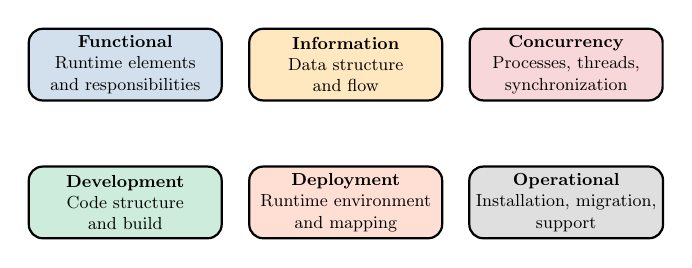
\begin{tikzpicture}[
    scale=0.7,
    transform shape,
    viewpoint/.style={draw, thick, fill=#1, minimum width=3.5cm, minimum height=1.3cm, rounded corners=5pt, font=\small, align=center}
]
    % Viewpoints in a grid
    \node[viewpoint=funccolor!25] (func) at (-4,2) {\textbf{Functional}\\Runtime elements\\and responsibilities};
    \node[viewpoint=infocolor!25] (info) at (0,2) {\textbf{Information}\\Data structure\\and flow};
    \node[viewpoint=conccolor!20] (conc) at (4,2) {\textbf{Concurrency}\\Processes, threads,\\synchronization};
    
    \node[viewpoint=devcolor!25] (dev) at (-4,-0.5) {\textbf{Development}\\Code structure\\and build};
    \node[viewpoint=deploycolor!25] (deploy) at (0,-0.5) {\textbf{Deployment}\\Runtime environment\\and mapping};
    \node[viewpoint=opscolor!25] (ops) at (4,-0.5) {\textbf{Operational}\\Installation, migration,\\support};
\end{tikzpicture}
\caption{Rozanski \& Woods Six Viewpoints}
\end{figure}

\begin{longtable}{@{}L{2.5cm} L{4cm} L{6cm}@{}}
\caption{R\&W Viewpoints Summary} \\
\toprule
\textbf{Viewpoint} & \textbf{Primary Concerns} & \textbf{Typical Models} \\
\midrule
\endfirsthead
\bottomrule
\endlastfoot
Functional & Functional capabilities; external interfaces; internal structure & Functional structure model; Component diagram \\
Information & Data structure; data flow; data ownership; data quality & Static data structure; Data flow; Data lifecycle \\
Concurrency & Task structure; process mapping; synchronization & Concurrency model; State model; Process diagram \\
Development & Module organization; codeline; common design & Module structure; Codeline model; Common design \\
Deployment & Runtime platform; network; technology dependencies & Deployment model; Network model; Technology model \\
Operational & Installation; migration; configuration; support & Installation model; Migration model; Config model \\
\end{longtable}

\subsection{Rozanski \& Woods Perspectives}

R\&W perspectives address cross-cutting quality concerns:

\begin{longtable}{@{}L{3cm} L{4.5cm} L{5cm}@{}}
\caption{R\&W Perspectives} \\
\toprule
\textbf{Perspective} & \textbf{Concerns} & \textbf{Applicable Viewpoints} \\
\midrule
\endfirsthead
\bottomrule
\endlastfoot
Security & Authentication; authorization; confidentiality; integrity & All viewpoints \\
Performance \& Scalability & Response time; throughput; scalability & Functional, Concurrency, Deployment \\
Availability \& Resilience & Availability; reliability; recovery; resilience & Functional, Concurrency, Deployment \\
Evolution & Dimensions of change; magnitude; likelihood & Development, Deployment \\
Location & Geographic distribution; data location & Deployment, Information \\
Development Resource & Team skills; schedule; budget & Development \\
Internationalization & Language; locale; cultural & Information, Functional \\
Accessibility & Disability access; usability & Functional \\
Regulation & Compliance; audit; legal & All viewpoints \\
Usability & Ease of use; learnability & Functional \\
\end{longtable}

\subsection{Views and Beyond Structure}

V\&B organizes views into three categories:

\begin{figure}[H]
\centering
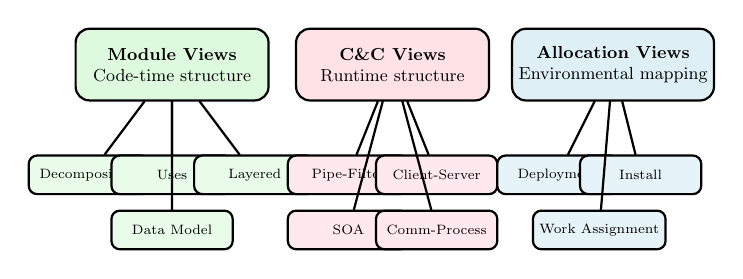
\begin{tikzpicture}[
    scale=0.7,
    transform shape,
    category/.style={draw, thick, fill=#1, minimum width=3.5cm, minimum height=1.3cm, rounded corners=5pt, font=\small, align=center},
    style/.style={draw, thick, fill=#1, minimum width=2.2cm, minimum height=0.7cm, rounded corners=3pt, font=\scriptsize, align=center}
]
    % Categories
    \node[category=modulecolor!30] (mod) at (-4,3) {\textbf{Module Views}\\Code-time structure};
    \node[category=cnccolor!40] (cnc) at (0,3) {\textbf{C\&C Views}\\Runtime structure};
    \node[category=alloccolor!40] (alloc) at (4,3) {\textbf{Allocation Views}\\Environmental mapping};
    
    % Styles under Module
    \node[style=modulecolor!20] (decomp) at (-5.5,1) {Decomposition};
    \node[style=modulecolor!20] (uses) at (-4,1) {Uses};
    \node[style=modulecolor!20] (layer) at (-2.5,1) {Layered};
    \node[style=modulecolor!20] (data) at (-4,0) {Data Model};
    
    % Styles under C&C
    \node[style=cnccolor!30] (pipe) at (-0.8,1) {Pipe-Filter};
    \node[style=cnccolor!30] (cs) at (0.8,1) {Client-Server};
    \node[style=cnccolor!30] (soa) at (-0.8,0) {SOA};
    \node[style=cnccolor!30] (comm) at (0.8,0) {Comm-Process};
    
    % Styles under Allocation
    \node[style=alloccolor!30] (deploy) at (3,1) {Deployment};
    \node[style=alloccolor!30] (install) at (4.5,1) {Install};
    \node[style=alloccolor!30] (work) at (3.75,0) {Work Assignment};
    
    % Connections
    \draw[thick] (mod) -- (decomp);
    \draw[thick] (mod) -- (uses);
    \draw[thick] (mod) -- (layer);
    \draw[thick] (mod) -- (data);
    \draw[thick] (cnc) -- (pipe);
    \draw[thick] (cnc) -- (cs);
    \draw[thick] (cnc) -- (soa);
    \draw[thick] (cnc) -- (comm);
    \draw[thick] (alloc) -- (deploy);
    \draw[thick] (alloc) -- (install);
    \draw[thick] (alloc) -- (work);
\end{tikzpicture}
\caption{Views and Beyond Structure}
\end{figure}

%==============================================================================
\section{Functional Viewpoint Mapping}
%==============================================================================

\begin{rwbox}[R\&W Functional Viewpoint]
\textbf{Purpose:} Describes the system's runtime functional elements and their responsibilities, interfaces, and primary interactions.

\textbf{Concerns Addressed:}
\begin{itemize}[nosep]
    \item Functional capabilities
    \item External interfaces
    \item Internal structure
    \item Functional design philosophy
\end{itemize}

\textbf{Models:}
\begin{itemize}[nosep]
    \item Functional Structure Model
    \item External Interface Model
    \item Component diagrams
\end{itemize}

\textbf{Stakeholders:} All stakeholders; particularly users, acquirers, developers, testers
\end{rwbox}

\begin{vbbox}[Views and Beyond Equivalent]
\textbf{Primary Mapping:} Component-and-Connector (C\&C) View Styles

The Functional viewpoint maps to one or more C\&C styles in V\&B:

\begin{itemize}
    \item \textbf{Client-Server Style:} For request-response interactions
    \item \textbf{Service-Oriented Style:} For service-based architectures
    \item \textbf{Pipe-and-Filter Style:} For data transformation pipelines
    \item \textbf{Publish-Subscribe Style:} For event-driven systems
    \item \textbf{Shared-Data Style:} For repository-centered systems
\end{itemize}

\textbf{Why C\&C:} Both the Functional viewpoint and C\&C views focus on runtime structure, component responsibilities, and interactions.
\end{vbbox}

\begin{mappingbox}[Implementation Mapping for Functional Viewpoint]

\textbf{R\&W Functional Structure Model} $\rightarrow$ \textbf{V\&B C\&C Primary Presentation}
\begin{itemize}[nosep]
    \item Functional elements $\rightarrow$ Components
    \item Interfaces $\rightarrow$ Ports
    \item Interactions $\rightarrow$ Connectors
    \item Responsibilities $\rightarrow$ Element catalog properties
\end{itemize}

\textbf{R\&W External Interface Model} $\rightarrow$ \textbf{V\&B Context Diagram + Interface Documentation}
\begin{itemize}[nosep]
    \item External entities $\rightarrow$ Context diagram actors
    \item Interface specifications $\rightarrow$ Interface documentation template
\end{itemize}

\textbf{R\&W Concerns} $\rightarrow$ \textbf{V\&B Documentation}
\begin{itemize}[nosep]
    \item Functional capabilities $\rightarrow$ Element catalog responsibilities
    \item Design philosophy $\rightarrow$ Rationale documentation
\end{itemize}
\end{mappingbox}

\begin{example}
\textbf{Functional View Mapping Example}

\textbf{R\&W Functional Element:}
\begin{quote}
``OrderProcessor: Receives customer orders, validates them, calculates pricing, and submits to fulfillment.''
\end{quote}

\textbf{V\&B C\&C Element Catalog Entry:}

\textit{Element:} OrderProcessor (Component)

\textit{Responsibilities:} Order validation; Pricing calculation; Fulfillment submission

\textit{Interfaces:}
\begin{itemize}[nosep]
    \item OrderSubmission (provided): Accepts customer orders
    \item FulfillmentRequest (required): Submits to fulfillment system
\end{itemize}

\textit{Quality Attributes:} Process 100 orders/second; 99.9\% availability
\end{example}

%==============================================================================
\section{Information Viewpoint Mapping}
%==============================================================================

\begin{rwbox}[R\&W Information Viewpoint]
\textbf{Purpose:} Describes the way the system stores, manipulates, manages, and distributes information.

\textbf{Concerns Addressed:}
\begin{itemize}[nosep]
    \item Data structure and content
    \item Data flow
    \item Data ownership and management
    \item Data quality (timeliness, availability, accuracy)
    \item Data volumes
\end{itemize}

\textbf{Models:}
\begin{itemize}[nosep]
    \item Static Data Structure Model (entities and relationships)
    \item Data Flow Model
    \item Data Ownership Model
    \item Data Lifecycle Model
\end{itemize}

\textbf{Stakeholders:} Users, developers, DBAs, compliance officers
\end{rwbox}

\begin{vbbox}[Views and Beyond Equivalent]
\textbf{Primary Mapping:} Data Model Style (Module Views) + C\&C Styles for Flow

\begin{itemize}
    \item \textbf{Data Model Style:} For static data structure (entities, relationships, attributes)
    \item \textbf{Shared-Data C\&C Style:} For data stores and accessor components
    \item \textbf{Pipe-and-Filter C\&C Style:} For data flow and transformations
    \item \textbf{Repository C\&C Style:} For centralized data management
\end{itemize}

\textbf{Additional V\&B Support:}
\begin{itemize}
    \item Interface documentation for data contracts
    \item Quality attribute scenarios for data quality
    \item Rationale for data ownership decisions
\end{itemize}
\end{vbbox}

\begin{mappingbox}[Implementation Mapping for Information Viewpoint]

\textbf{R\&W Static Data Structure} $\rightarrow$ \textbf{V\&B Data Model View}
\begin{itemize}[nosep]
    \item Entities $\rightarrow$ Data entities in data model
    \item Relationships $\rightarrow$ Relations in data model
    \item Attributes $\rightarrow$ Entity properties
\end{itemize}

\textbf{R\&W Data Flow Model} $\rightarrow$ \textbf{V\&B C\&C View (Pipe-Filter or Shared-Data)}
\begin{itemize}[nosep]
    \item Data flows $\rightarrow$ Connectors with data semantics
    \item Transformation points $\rightarrow$ Filter components
    \item Data stores $\rightarrow$ Repository components
\end{itemize}

\textbf{R\&W Data Ownership} $\rightarrow$ \textbf{V\&B Element Catalog + Rationale}
\begin{itemize}[nosep]
    \item Ownership assignments $\rightarrow$ Element properties
    \item Ownership rationale $\rightarrow$ Rationale documentation
\end{itemize}

\textbf{R\&W Data Quality Concerns} $\rightarrow$ \textbf{V\&B Quality Attribute Scenarios}
\begin{itemize}[nosep]
    \item Timeliness $\rightarrow$ Performance scenarios
    \item Availability $\rightarrow$ Availability scenarios
    \item Accuracy $\rightarrow$ Integrity requirements
\end{itemize}
\end{mappingbox}

%==============================================================================
\section{Concurrency Viewpoint Mapping}
%==============================================================================

\begin{rwbox}[R\&W Concurrency Viewpoint]
\textbf{Purpose:} Describes the concurrency structure of the system and maps functional elements to concurrency units.

\textbf{Concerns Addressed:}
\begin{itemize}[nosep]
    \item Task structure
    \item Mapping of functional elements to tasks
    \item Interprocess communication
    \item State management
    \item Synchronization and integrity
    \item Startup, shutdown, and failure behavior
\end{itemize}

\textbf{Models:}
\begin{itemize}[nosep]
    \item System-level Concurrency Model
    \item State Model
    \item Process Structure Diagram
\end{itemize}

\textbf{Stakeholders:} Developers, testers, performance engineers, operations
\end{rwbox}

\begin{vbbox}[Views and Beyond Equivalent]
\textbf{Primary Mapping:} Communicating-Processes C\&C Style

The V\&B Communicating-Processes style directly addresses concurrency:

\begin{itemize}
    \item \textbf{Elements:} Processes, threads, or concurrent units
    \item \textbf{Connectors:} Communication mechanisms (synchronous, asynchronous, shared memory)
    \item \textbf{Properties:} Thread safety, synchronization, scheduling
\end{itemize}

\textbf{Additional V\&B Support:}
\begin{itemize}
    \item Behavior documentation for state transitions
    \item Sequence diagrams for interaction scenarios
    \item Quality attribute scenarios for performance
\end{itemize}
\end{vbbox}

\begin{mappingbox}[Implementation Mapping for Concurrency Viewpoint]

\textbf{R\&W Concurrency Model} $\rightarrow$ \textbf{V\&B Communicating-Processes C\&C View}
\begin{itemize}[nosep]
    \item Tasks/Processes $\rightarrow$ Process components
    \item Interprocess communication $\rightarrow$ Connector types
    \item Synchronization $\rightarrow$ Connector properties
\end{itemize}

\textbf{R\&W State Model} $\rightarrow$ \textbf{V\&B Behavior Documentation}
\begin{itemize}[nosep]
    \item State diagrams $\rightarrow$ Behavior documentation within C\&C view
    \item State transitions $\rightarrow$ State machine notation
\end{itemize}

\textbf{R\&W Task Mapping} $\rightarrow$ \textbf{V\&B View Mapping}
\begin{itemize}[nosep]
    \item Functional-to-task mapping $\rightarrow$ Mapping between C\&C views
\end{itemize}
\end{mappingbox}

%==============================================================================
\section{Development Viewpoint Mapping}
%==============================================================================

\begin{rwbox}[R\&W Development Viewpoint]
\textbf{Purpose:} Describes the architecture that supports the software development process.

\textbf{Concerns Addressed:}
\begin{itemize}[nosep]
    \item Module organization
    \item Common processing (shared code)
    \item Standardization of design
    \item Standardization of testing
    \item Codeline organization
    \item Build and configuration management
\end{itemize}

\textbf{Models:}
\begin{itemize}[nosep]
    \item Module Structure Model
    \item Common Design Model
    \item Codeline Model
\end{itemize}

\textbf{Stakeholders:} Developers, testers, build engineers, maintainers
\end{rwbox}

\begin{vbbox}[Views and Beyond Equivalent]
\textbf{Primary Mapping:} Module View Styles + Documentation Beyond Views

\begin{itemize}
    \item \textbf{Decomposition Style:} For module structure (hierarchy of modules)
    \item \textbf{Layered Style:} For layer structure and dependencies
    \item \textbf{Uses Style:} For module dependencies and allowed usage
    \item \textbf{Implementation/Install Style:} For codeline model
\end{itemize}

\textbf{Additional V\&B Support:}
\begin{itemize}
    \item Rationale for common design decisions
    \item Documentation beyond views for conventions
    \item Work Assignment view for team structure
\end{itemize}
\end{vbbox}

\begin{mappingbox}[Implementation Mapping for Development Viewpoint]

\textbf{R\&W Module Structure Model} $\rightarrow$ \textbf{V\&B Decomposition/Layered View}
\begin{itemize}[nosep]
    \item Modules $\rightarrow$ Modules in decomposition
    \item Layers $\rightarrow$ Layers in layered view
    \item Dependencies $\rightarrow$ Uses relations
\end{itemize}

\textbf{R\&W Common Design Model} $\rightarrow$ \textbf{V\&B Documentation Beyond Views}
\begin{itemize}[nosep]
    \item Common patterns $\rightarrow$ Design guidance in rationale
    \item Design conventions $\rightarrow$ Documented in system overview
    \item Shared assumptions $\rightarrow$ Documented assumptions
\end{itemize}

\textbf{R\&W Codeline Model} $\rightarrow$ \textbf{V\&B Implementation/Install Style}
\begin{itemize}[nosep]
    \item Source structure $\rightarrow$ Implementation view
    \item Build organization $\rightarrow$ Install view
    \item Configuration management $\rightarrow$ Documentation beyond views
\end{itemize}
\end{mappingbox}

%==============================================================================
\section{Deployment Viewpoint Mapping}
%==============================================================================

\begin{rwbox}[R\&W Deployment Viewpoint]
\textbf{Purpose:} Describes the environment into which the system will be deployed and the dependencies the system has on its runtime environment.

\textbf{Concerns Addressed:}
\begin{itemize}[nosep]
    \item Runtime platform requirements
    \item Hardware requirements
    \item Network requirements
    \item Technology compatibility
    \item Network capacity
\end{itemize}

\textbf{Models:}
\begin{itemize}[nosep]
    \item Runtime Platform Model
    \item Network Model
    \item Technology Dependency Model
\end{itemize}

\textbf{Stakeholders:} Operations, developers, system administrators, acquirers
\end{rwbox}

\begin{vbbox}[Views and Beyond Equivalent]
\textbf{Primary Mapping:} Deployment Style (Allocation Views) + Uses Style

\begin{itemize}
    \item \textbf{Deployment Style:} For runtime platform and network models
    \begin{itemize}[nosep]
        \item Software elements mapped to hardware nodes
        \item Network topology
        \item Resource allocation
    \end{itemize}
    \item \textbf{Uses Style:} For technology dependency model
    \begin{itemize}[nosep]
        \item Dependencies on runtime environment
        \item Library and framework dependencies
    \end{itemize}
\end{itemize}
\end{vbbox}

\begin{mappingbox}[Implementation Mapping for Deployment Viewpoint]

\textbf{R\&W Runtime Platform Model} $\rightarrow$ \textbf{V\&B Deployment View}
\begin{itemize}[nosep]
    \item Processing nodes $\rightarrow$ Deployment nodes
    \item Software-to-hardware mapping $\rightarrow$ Allocation relations
    \item Resource requirements $\rightarrow$ Node properties
\end{itemize}

\textbf{R\&W Network Model} $\rightarrow$ \textbf{V\&B Deployment View}
\begin{itemize}[nosep]
    \item Network topology $\rightarrow$ Node connections
    \item Network properties $\rightarrow$ Connection properties
    \item Network segments $\rightarrow$ Environmental regions
\end{itemize}

\textbf{R\&W Technology Dependency Model} $\rightarrow$ \textbf{V\&B Uses View + Element Catalog}
\begin{itemize}[nosep]
    \item Technology dependencies $\rightarrow$ Uses relations
    \item Version requirements $\rightarrow$ Element catalog properties
    \item Compatibility constraints $\rightarrow$ Variability guide
\end{itemize}
\end{mappingbox}

%==============================================================================
\section{Operational Viewpoint Mapping}
%==============================================================================

\begin{rwbox}[R\&W Operational Viewpoint]
\textbf{Purpose:} Describes how the system will be operated, administered, and supported when running in production.

\textbf{Concerns Addressed:}
\begin{itemize}[nosep]
    \item Installation and upgrade
    \item Functional migration
    \item Data migration
    \item Operational monitoring and control
    \item Configuration management
    \item Support and maintenance
\end{itemize}

\textbf{Models:}
\begin{itemize}[nosep]
    \item Installation Model
    \item Migration Model
    \item Configuration Model
    \item Administration Model
    \item Support Model
\end{itemize}

\textbf{Stakeholders:} Operations, system administrators, support staff, maintainers
\end{rwbox}

\begin{vbbox}[Views and Beyond Equivalent]
\textbf{Primary Mapping:} Install Style + Documentation Beyond Views

\begin{itemize}
    \item \textbf{Install Style:} For installation model
    \begin{itemize}[nosep]
        \item File system structure
        \item Configuration locations
        \item Installation procedures
    \end{itemize}
    \item \textbf{Documentation Beyond Views:} For operational requirements and solutions
    \begin{itemize}[nosep]
        \item Operational procedures in system overview
        \item Migration plans in rationale
        \item Configuration guidance
    \end{itemize}
\end{itemize}

Operational concerns can be associated with any view where solutions are documented.
\end{vbbox}

\begin{mappingbox}[Implementation Mapping for Operational Viewpoint]

\textbf{R\&W Installation Model} $\rightarrow$ \textbf{V\&B Install View}
\begin{itemize}[nosep]
    \item Installation structure $\rightarrow$ Install view primary presentation
    \item Installation procedures $\rightarrow$ Associated documentation
\end{itemize}

\textbf{R\&W Migration Model} $\rightarrow$ \textbf{V\&B Documentation Beyond Views}
\begin{itemize}[nosep]
    \item Migration strategy $\rightarrow$ Rationale / system overview
    \item Migration procedures $\rightarrow$ Operational documentation
\end{itemize}

\textbf{R\&W Configuration Model} $\rightarrow$ \textbf{V\&B Variability Guide + Install View}
\begin{itemize}[nosep]
    \item Configuration options $\rightarrow$ Variability guide
    \item Configuration locations $\rightarrow$ Install view
\end{itemize}

\textbf{R\&W Operations Concerns} $\rightarrow$ \textbf{V\&B View Annotations}
\begin{itemize}[nosep]
    \item Monitoring requirements $\rightarrow$ C\&C view properties
    \item Administration requirements $\rightarrow$ Deployment view properties
    \item Support requirements $\rightarrow$ Documentation beyond views
\end{itemize}
\end{mappingbox}

%==============================================================================
\section{Perspectives and Quality Attributes}
%==============================================================================

\subsection{Mapping Perspectives to V\&B Approaches}

R\&W perspectives are cross-cutting concerns that apply across viewpoints. V\&B addresses these through quality attribute analysis.

\begin{longtable}{@{}L{3cm} L{4cm} L{5.5cm}@{}}
\caption{Perspective to V\&B Mapping} \\
\toprule
\textbf{R\&W Perspective} & \textbf{V\&B Approach} & \textbf{Documentation Location} \\
\midrule
\endfirsthead
\toprule
\textbf{R\&W Perspective} & \textbf{V\&B Approach} & \textbf{Documentation Location} \\
\midrule
\endhead
\bottomrule
\endlastfoot
Security & Security tactics; Security view & C\&C view; Deployment view; Rationale \\
Performance \& Scalability & Performance scenarios; Performance tactics & C\&C view properties; Rationale \\
Availability \& Resilience & Availability scenarios; Tactics & C\&C view; Deployment view; Behavior \\
Evolution & Modifiability scenarios; Variability & Variability guide; Rationale \\
Location & Deployment allocation & Deployment view \\
Development Resource & Work assignment & Work Assignment view \\
Internationalization & Data model; Configuration & Data model view; Variability guide \\
Accessibility & Functional requirements & C\&C view; Interface documentation \\
Regulation & Constraints; Compliance & Rationale; Constraints documentation \\
Usability & Functional requirements & C\&C view; Interface documentation \\
\end{longtable}

\subsection{Security Perspective}

\begin{perspbox}[Security Perspective Mapping]
\textbf{R\&W Security Concerns:}
\begin{itemize}[nosep]
    \item Authentication and authorization
    \item Confidentiality and integrity
    \item Non-repudiation and audit
    \item Threat identification
\end{itemize}

\textbf{V\&B Documentation Approach:}
\begin{itemize}
    \item \textbf{C\&C View:} Security components (authentication services, encryption services)
    \item \textbf{Deployment View:} Security zones, network segmentation, firewall placement
    \item \textbf{Rationale:} Security decisions and threat analysis
    \item \textbf{Quality Scenarios:} Security-specific scenarios (e.g., ``Attacker attempts SQL injection; system detects and blocks within 1 second'')
\end{itemize}
\end{perspbox}

\subsection{Performance and Scalability Perspective}

\begin{perspbox}[Performance \& Scalability Perspective Mapping]
\textbf{R\&W Performance Concerns:}
\begin{itemize}[nosep]
    \item Response time and throughput
    \item Scalability dimensions
    \item Resource utilization
    \item Peak load handling
\end{itemize}

\textbf{V\&B Documentation Approach:}
\begin{itemize}
    \item \textbf{C\&C View:} Performance-critical components; Connector properties (latency, bandwidth)
    \item \textbf{Deployment View:} Resource allocation; Scaling units
    \item \textbf{Element Catalog:} Performance properties per element
    \item \textbf{Quality Scenarios:} Performance scenarios with specific measures
    \item \textbf{Rationale:} Performance tactics applied and tradeoffs made
\end{itemize}
\end{perspbox}

\subsection{Availability and Resilience Perspective}

\begin{perspbox}[Availability \& Resilience Perspective Mapping]
\textbf{R\&W Availability Concerns:}
\begin{itemize}[nosep]
    \item Availability targets
    \item Failure detection and recovery
    \item Redundancy and failover
    \item Disaster recovery
\end{itemize}

\textbf{V\&B Documentation Approach:}
\begin{itemize}
    \item \textbf{C\&C View:} Redundant components; Health monitoring; Circuit breakers
    \item \textbf{Deployment View:} Redundancy placement; Failover paths; Disaster recovery sites
    \item \textbf{Behavior Documentation:} Failure scenarios; Recovery procedures
    \item \textbf{Quality Scenarios:} Availability scenarios (e.g., ``Database fails; system recovers within 30 seconds'')
\end{itemize}
\end{perspbox}

%==============================================================================
\section{Complete Mapping Reference}
%==============================================================================

\begin{longtable}{@{}L{3cm} L{4.5cm} L{5cm}@{}}
\caption{Complete Viewpoint Mapping Reference} \\
\toprule
\textbf{R\&W Viewpoint} & \textbf{V\&B View Type(s)} & \textbf{Implementation Notes} \\
\midrule
\endfirsthead
\toprule
\textbf{R\&W Viewpoint} & \textbf{V\&B View Type(s)} & \textbf{Implementation Notes} \\
\midrule
\endhead
\bottomrule
\endlastfoot

\multicolumn{3}{l}{\textbf{Functional Viewpoint}} \\
\quad Functional Structure & C\&C Views (Client-Server, SOA, Pipe-Filter) & Choose style based on interaction patterns \\
\quad External Interfaces & Context Diagram + Interface Documentation & Use V\&B interface template \\
\quad Design Philosophy & Rationale Documentation & Document in system overview \\
\midrule

\multicolumn{3}{l}{\textbf{Information Viewpoint}} \\
\quad Static Data Structure & Data Model View & Entity-relationship notation \\
\quad Data Flow & C\&C View (Pipe-Filter, Shared-Data) & Document data semantics on connectors \\
\quad Data Ownership & Element Catalog Properties & Document in data model view \\
\quad Data Quality & Quality Attribute Scenarios & Create data-specific scenarios \\
\midrule

\multicolumn{3}{l}{\textbf{Concurrency Viewpoint}} \\
\quad Concurrency Model & C\&C View (Communicating-Processes) & Document processes, synchronization \\
\quad State Model & Behavior Documentation & State diagrams within C\&C view \\
\quad Task Mapping & View Mapping & Map functional to concurrency views \\
\midrule

\multicolumn{3}{l}{\textbf{Development Viewpoint}} \\
\quad Module Structure & Decomposition View, Layered View & Use for code organization \\
\quad Common Design & Documentation Beyond Views & Document patterns, conventions \\
\quad Codeline Model & Implementation/Install View & Source structure, build \\
\midrule

\multicolumn{3}{l}{\textbf{Deployment Viewpoint}} \\
\quad Runtime Platform & Deployment View & Software-to-hardware mapping \\
\quad Network Model & Deployment View & Node connections, topology \\
\quad Technology Dependencies & Uses View & Dependencies on environment \\
\midrule

\multicolumn{3}{l}{\textbf{Operational Viewpoint}} \\
\quad Installation Model & Install View & File structure, config locations \\
\quad Migration Model & Documentation Beyond Views & Migration strategy in rationale \\
\quad Configuration Model & Variability Guide & Configuration options \\
\quad Operations Concerns & View Annotations & Annotate relevant views \\

\end{longtable}

%==============================================================================
\section{Implementation Guidance}
%==============================================================================

\subsection{Creating Integrated Documentation}

\begin{bestpractice}
\textbf{Integration Strategy:}

\begin{enumerate}
    \item \textbf{Start with stakeholder analysis:} Identify stakeholders familiar with each framework
    
    \item \textbf{Map required content:} Determine which R\&W viewpoints are needed and map to V\&B views
    
    \item \textbf{Choose primary organization:} Decide whether to organize by R\&W viewpoints or V\&B categories
    
    \item \textbf{Create cross-references:} Provide navigation aids for stakeholders familiar with either framework
    
    \item \textbf{Document perspectives/quality attributes:} Ensure cross-cutting concerns are addressed in appropriate views
\end{enumerate}
\end{bestpractice}

\subsection{Documentation Structure Options}

\begin{longtable}{@{}L{3cm} L{4cm} L{5.5cm}@{}}
\caption{Documentation Organization Options} \\
\toprule
\textbf{Approach} & \textbf{Organization} & \textbf{When to Use} \\
\midrule
\endfirsthead
\bottomrule
\endlastfoot
R\&W Primary & Organize by R\&W viewpoints; note V\&B equivalents & Stakeholders familiar with R\&W; need viewpoint structure \\
V\&B Primary & Organize by V\&B categories; note R\&W coverage & Stakeholders familiar with V\&B; SEI-aligned projects \\
Hybrid & Use V\&B structure with R\&W viewpoint mapping & Mixed stakeholder community; need both frameworks \\
Concern-Driven & Organize by stakeholder concerns; map to both & Custom organization; highly diverse stakeholders \\
\end{longtable}

\subsection{View Packet Design}

When creating view packets that satisfy both frameworks:

\begin{checklistbox}[View Packet Completeness Checklist]
\textbf{For V\&B Completeness:}
\begin{itemize}[leftmargin=1.5cm]
    \item[$\square$] Primary presentation (diagram)
    \item[$\square$] Element catalog
    \item[$\square$] Context diagram (if applicable)
    \item[$\square$] Variability guide
    \item[$\square$] Rationale
    \item[$\square$] Behavior documentation (if applicable)
\end{itemize}

\textbf{For R\&W Viewpoint Coverage:}
\begin{itemize}[leftmargin=1.5cm]
    \item[$\square$] All viewpoint concerns addressed
    \item[$\square$] Required models included
    \item[$\square$] Stakeholder needs met
    \item[$\square$] Problems/pitfalls considered
\end{itemize}

\textbf{For Perspective/Quality Attribute Coverage:}
\begin{itemize}[leftmargin=1.5cm]
    \item[$\square$] Cross-cutting concerns documented
    \item[$\square$] Quality scenarios defined
    \item[$\square$] Tactics documented in rationale
\end{itemize}
\end{checklistbox}

%==============================================================================
\section{Appendix A: Quick Reference Mapping}
%==============================================================================

\begin{longtable}{@{}L{4cm} L{8.5cm}@{}}
\caption{Quick Reference: R\&W to V\&B Mapping} \\
\toprule
\textbf{R\&W View/Model} & \textbf{V\&B Approach} \\
\midrule
\endfirsthead
\bottomrule
\endlastfoot
Functional View & One or more C\&C styles \\
Information View (Structure) & Data Model style \\
Information View (Flow) & C\&C style (Pipe-Filter, Shared-Data) \\
Concurrency View & C\&C Communicating-Processes style \\
Development View (Structure) & Decomposition or Layered style \\
Development View (Codeline) & Implementation/Install style \\
Development View (Common Design) & Documentation beyond views \\
Deployment View (Platform) & Deployment style \\
Deployment View (Network) & Deployment style \\
Deployment View (Technology) & Uses style \\
Operational View (Installation) & Install style \\
Operational View (Operations) & Documentation beyond views \\
\midrule
Security Perspective & Security annotations in C\&C/Deployment; Rationale \\
Performance Perspective & Performance properties; Quality scenarios; Rationale \\
Availability Perspective & Availability tactics in views; Quality scenarios \\
Evolution Perspective & Variability guide; Modifiability scenarios \\
\end{longtable}

%==============================================================================
\section{Appendix B: Glossary}
%==============================================================================

\begin{description}[leftmargin=3cm, style=nextline]
    \item[C\&C View] Component-and-Connector view; shows runtime structure
    \item[Concern] Stakeholder interest in the system
    \item[Element Catalog] Detailed specification of view elements
    \item[Module View] View showing code-time structure
    \item[Perspective] R\&W cross-cutting quality concern
    \item[Quality Attribute] Measurable system property (performance, security, etc.)
    \item[Style] V\&B term for a type of view with specific element/relation types
    \item[View] Work product expressing architecture for specific concerns
    \item[View Packet] V\&B unit of view documentation
    \item[Viewpoint] Conventions for constructing and interpreting views
\end{description}

%==============================================================================
\section{Appendix C: References}
%==============================================================================

\begin{enumerate}
    \item Rozanski, N., \& Woods, E. (2011). \textit{Software Systems Architecture: Working with Stakeholders Using Viewpoints and Perspectives} (2nd ed.). Addison-Wesley.
    
    \item Clements, P., et al. (2010). \textit{Documenting Software Architectures: Views and Beyond} (2nd ed.). Addison-Wesley.
    
    \item Bass, L., Clements, P., \& Kazman, R. (2021). \textit{Software Architecture in Practice} (4th ed.). Addison-Wesley.
    
    \item ISO/IEC/IEEE 42010:2011. \textit{Systems and software engineering---Architecture description}.
    
    \item Kruchten, P. (1995). ``The 4+1 View Model of Architecture.'' \textit{IEEE Software}, 12(6), 42-50.
    
    \item IEEE 1471-2000. \textit{IEEE Recommended Practice for Architectural Description of Software-Intensive Systems}.
    
    \item Hofmeister, C., Nord, R., \& Soni, D. (2000). \textit{Applied Software Architecture}. Addison-Wesley.
    
    \item Garlan, D. (2003). ``Formal Modeling and Analysis of Software Architecture.'' \textit{Formal Methods for Software Architectures}, LNCS 2804.
\end{enumerate}

\end{document}
